% =============================================================================
\bloco{1}{Foundations: AD, AS, natural and efficient output, taxes}{Benigno \S\S1--5 \,\textbullet\, 25 points}

\questao{(10 points) Objective items.}

\textbf{a)} (3 points) The slope $\kappa$ of the AS curve $p-p^e=\kappa(y-y_n)$, in terms of the primitives, is:
\begin{alternativas}
\item $(1-\alpha)(\sigma^{-1}+\eta)$
\item $\alpha(\sigma^{-1}+\eta)/(1-\alpha)$
\item $(1-\alpha)(\sigma+\eta)$
\item $(1-\alpha)(\sigma^{-1}+\eta)/\alpha$
\end{alternativas}
\gabarito{D}
\begin{sol}
\passo{derivation}{Flexible firms set $\tilde p=w-a+\mu$, a markup over marginal cost $W/A$. Labor supply in logs, $w-p=\eta l+\tilde\sigma^{-1}c$,
with $l=y-a$ (technology) and $c=(y-g)/s_c$ (resources), reads $w-p=\eta(y-a)+\sigma^{-1}(y-g)$, so $\tilde p-p=(\sigma^{-1}+\eta)(y-y_n)$.
Aggregating, $p-p^e=(1-\alpha)[(\tilde p-p)+(p-p^e)]$, i.e.\ $\alpha(p-p^e)=(1-\alpha)(\sigma^{-1}+\eta)(y-y_n)$.}
\passo{distractors}{A drops the feedback of $p$ on the flexible firms' relative price, writing $p-p^e=(1-\alpha)(\tilde p-p)$; B swaps the
weights of preset and flexible prices; C makes two mistakes: it drops the feedback, as A does, and reads $\sigma$ as the curvature of
utility, not the elasticity of substitution.}
\refbib{Benigno (2015), \S4.1, eqs.\ (11)--(17), pp.~507--508.}
\end{sol}

\medskip
\textbf{b)} (3 points) \emph{AS--AD $\times$ taxation.} Short-run productivity rises ($a>0$) and a payroll tax raises the (log) markup
by $\mu>0$, both temporarily. The changes in natural and efficient output, $(\Delta y_n,\,\Delta y_e)$, are:
\begin{alternativas}
\item $\bigl((a-\mu)/(\sigma^{-1}+\eta),\ a/(\sigma^{-1}+\eta)\bigr)$
\item $\bigl([(1+\eta)a-\mu]/(\sigma^{-1}+\eta),\ (1+\eta)a/(\sigma^{-1}+\eta)\bigr)$
\item $\bigl([(1+\eta)a-\mu]/(\sigma^{-1}+\eta),\ [(1+\eta)a-\mu]/(\sigma^{-1}+\eta)\bigr)$
\item $\bigl(a/(\sigma^{-1}+\eta),\ a/(\sigma^{-1}+\eta)\bigr)$
\end{alternativas}
\gabarito{B}
\begin{sol}
\passo{derivation}{Setting $\tilde p=p$ in the gap relation of (a): $(\sigma^{-1}+\eta)y_n=(1+\eta)a+\sigma^{-1}g-\mu$, and the payroll tax enters only
through the aggregate markup (eq.\ 13). The planner sets $v_l(Y/A)/u_c(Y-G)=A$, with no markup and no tax: $\sigma^{-1}(y-g)+\eta(y-a)=a$.
Productivity carries $1+\eta$ in both: it raises the marginal product ($a$) and saves hours ($l=y-a$).}
\passo{distractors}{A uses $l=y$ and loses the $\eta a$ term; C lets the planner face the tax; D makes two mistakes: it uses $l=y$, as A
does, and treats the rebated payroll tax as lump sum, so $\mu$ leaves $y_n$.}
\refbib{Benigno (2015), \S4.1, eqs.\ (13), (15), pp.~507--508; \S4.4, eq.\ (19), p.~509.}
\end{sol}

\medskip
\textbf{c)} (2 points, T or F) Because $\theta$ sets the markup, a higher demand elasticity $\theta$ makes the AS curve steeper.
\gabarito{F}
\begin{sol}
\passo{proof}{$\kappa=(1-\alpha)(\sigma^{-1}+\eta)/\alpha$ has no $\theta$. It would enter only if a firm's marginal cost depended on its own output
(decreasing returns, firm-specific labor: real rigidity); with $Y(j)=AL(j)$ and one labor market, marginal cost $W/A$ is common to
all firms. $\theta$ moves the level: $\mu_\theta=\ln\frac{\theta}{\theta-1}$ gives $\partial y_n/\partial\theta=\frac{1}{\theta(\theta-1)(\sigma^{-1}+\eta)}>0$, a parallel
shift of the AS. It reappears as the weight $\theta/\kappa$ on price stability in the loss function (33).}
\refbib{Benigno (2015), \S4.1, eqs.\ (13), (17), pp.~507--508; \S11, eq.\ (33), p.~521; Romer (2012), \S\S6.5 and 6.7.}
\end{sol}

\medskip
\textbf{d)} (2 points, T or F) \emph{AS--AD $\times$ fiscal news.} Holding $i$, $\bar p$ and $p^e$ fixed, news that long-run government
spending will be higher ($\bar g\uparrow$, $g$ unchanged) lowers current output.
\gabarito{T}
\begin{sol}
\passo{proof}{By (15), $\bar y_n-\bar g=\frac{(1+\eta)\bar a-\bar\mu-\eta\bar g}{\sigma^{-1}+\eta}$: long-run output absorbs only the share $\frac{\sigma^{-1}}{\sigma^{-1}+\eta}<1$
of $\bar g$, so long-run consumption falls and smoothing cuts current demand; the AS does not move ($y_n$ depends on current $g$
only). Solving AD and AS, $\frac{dy}{d\bar g}=-\frac{\eta}{(\sigma^{-1}+\eta)(1+\sigma\kappa)}=-m_{\bar g}<0$ for every $\eta>0$; it vanishes only as $\eta\to0$.}
\refbib{Benigno (2015), \S8, Table 1, p.~515.}
\end{sol}

% -----------------------------------------------------------------------------
\questao{(15 points) Discursive. \emph{AS--AD foundations $\times$ taxation $\times$ supply shocks.} Build the model from its
primitives (no taxes unless stated).}

\textbf{a)} (3 points) From the household problem with budget $PC+\frac{\bar P\bar C}{1+i}=WL+\frac{\bar W\bar L}{1+i}+T$, derive the
Euler equation and the labor-supply condition; log-linearize and combine with $y=s_cc+g$ to obtain the AD curve. Give
its slope in the $(y,p)$ plane, explain it, and sign the effect of each shifter.
\resolespaco
\begin{sol}
\passo{FOCs}{$\mathcal L=u(C)-v(L)+\beta[u(\bar C)-v(\bar L)]+\lambda\bigl[WL+\frac{\bar W\bar L}{1+i}+T-PC-\frac{\bar P\bar C}{1+i}\bigr]$, $\lambda$ the
marginal utility of nominal wealth: $u_c(C)=\lambda P$, $\beta u_c(\bar C)=\lambda\bar P/(1+i)$, $v_l(L)=\lambda W$. Dividing,
$\frac{u_c(C)}{\beta u_c(\bar C)}=(1+i)\frac P{\bar P}\equiv1+r$ (Euler) and $\frac{v_l(L)}{u_c(C)}=\frac WP$ (labor supply).}
\passo{log-linear Euler}{With $u_c=C^{-1/\tilde\sigma}$, $\ln(1+i)\approx i$ and $\rho=-\ln\beta$: $\bar c-c=\tilde\sigma[i-(\bar p-p)-\rho]$.}
\passo{AD}{Resources give $c=(y-g)/s_c$ and $\bar c=(\bar y-\bar g)/s_c$; long-run prices are flexible, $\bar y=\bar y_n$; and $\sigma=\tilde\sigma s_c$:
\[y=\bar y_n+(g-\bar g)-\sigma[i-(\bar p-p)-\rho].\]
Slope $dp/dy=-1/\sigma$: given $i$ and $\bar p$, a higher $p$ lowers expected inflation $\bar p-p$, raising the real rate and saving (an
intertemporal channel; no LM curve). Shifters: $\partial y/\partial i=-\sigma$, $\partial y/\partial g=1$, $\partial y/\partial\bar p=\sigma$ and, through $\bar y_n$ in (15),
$\partial y/\partial\bar a=\frac{1+\eta}{\sigma^{-1}+\eta}$, $\partial y/\partial\bar\mu=-\frac{1}{\sigma^{-1}+\eta}$, $\partial y/\partial\bar g=-\frac{\eta}{\sigma^{-1}+\eta}$.}
\intuicao{The AD is the Euler equation in output: higher expected income or a lower real rate raises demand today.}
\refbib{Benigno (2015), \S3, eqs.\ (1)--(6), pp.~505--506; \S5, eq.\ (21), p.~509; Kurlat (2020), \S6.2 and \S7.2.}
\rubrica{
\item FOCs with the meaning of $\lambda$: 1 pt.
\item Log-linear Euler: 1 pt. Quoted instead of derived: max.\ a third of the item.
\item AD, slope and mechanism, signed shifters: 1 pt; slope via money demand: 0 for this line.
}
\end{sol}

\textbf{b)} (3 points) From the firm's problem derive the optimal flexible price, natural output and the AS curve
with a fraction $\alpha$ of preset prices.
\resolespaco
\begin{sol}
\passo{optimal price}{$\Pi(j)=(P(j)-\frac WA)(\frac{P(j)}P)^{-\theta}(C+G)$ by demand (9) and technology; $\Pi'(P(j))$ has the sign of $(1-\theta)P(j)+\theta\frac WA$,
positive below and negative above $P(j)=\frac{\theta}{\theta-1}\frac WA$, the unique maximum ($\theta>1$). In logs $\tilde p=w-a+\mu$, $\mu=\ln\frac{\theta}{\theta-1}$.}
\passo{gap relation}{Labor supply from (a) in logs, $w-p=\eta(y-a)+\sigma^{-1}(y-g)$ (using $l=y-a$, $\tilde\sigma^{-1}c=\sigma^{-1}(y-g)$), gives
$\tilde p-p=(\sigma^{-1}+\eta)y-(1+\eta)a-\sigma^{-1}g+\mu=(\sigma^{-1}+\eta)(y-y_n)$, $y_n=\frac{(1+\eta)a+\sigma^{-1}g-\mu}{\sigma^{-1}+\eta}$: the output at which
flexible firms keep their relative price.}
\passo{AS}{$p=\alpha p^e+(1-\alpha)\tilde p$ gives $\alpha(p-p^e)=(1-\alpha)(\tilde p-p)$, so $p-p^e=\kappa(y-y_n)$, $\kappa=\frac{(1-\alpha)(\sigma^{-1}+\eta)}{\alpha}$, falling
in $\alpha$ from $\infty$ ($\alpha\to0$, vertical AS at $y_n$) to 0 ($\alpha\to1$, flat AS at $p^e$).}
\intuicao{Real marginal cost rises with $y-y_n$ through the real wage ($\eta$, $\sigma^{-1}$); the $1-\alpha$ flexible firms pass it into prices.}
\refbib{Benigno (2015), \S4.1, eqs.\ (9)--(17), pp.~506--508; Romer (2012), problem 6.16.}
\rubrica{
\item Optimal price with the second-order argument: 1 pt.
\item Gap relation and $y_n$: 1 pt.
\item AS and $\kappa$: 1 pt. $\kappa$ quoted: max.\ a third of the item.
}
\end{sol}

\textbf{c)} (3 points) Derive efficient output from the planner's problem and compare it with natural output. Show how
labor, payroll, sales and consumption taxes affect each, and find the sales subsidy that makes the steady state efficient.
How does it depend on $\theta$?
\resolespaco
\begin{sol}
\passo{planner}{$\max_Y u(Y-G)-v(Y/A)$ is strictly concave; in its FOC $u_c(Y-G)=v_l(Y/A)/A$ the left side falls from $\infty$ to 0 and the
right side rises without bound: one solution. In logs $\sigma^{-1}(y-g)+\eta(y-a)=a$, so $y_e=\frac{(1+\eta)a+\sigma^{-1}g}{\sigma^{-1}+\eta}$ and, by (b),
$y_n-y_e=-\frac{\mu}{\sigma^{-1}+\eta}<0$: the markup is a wedge between the marginal rate of substitution and the marginal product $A$.}
\passo{taxes}{Profits (10) give $P(j)=\frac{\theta}{\theta-1}\frac{1+\tau_w}{1-\tau_y}\frac WA$; labor supply (7) is $\frac{v_l}{u_c}=\frac{1-\tau_l}{1+\tau_c}\frac WP$. Eliminating
$W/P$ with $P(j)=P$: $\frac{v_l(Y_n/A)}{u_c(Y_n-G)}=Ae^{-\mu}$, with gross markup $e^{\mu}=\frac{\theta}{\theta-1}\frac{(1+\tau_w)(1+\tau_c)}{(1-\tau_y)(1-\tau_l)}$ (eq.\ 13; $\mu$ stays
the log markup, as in (b)), increasing in each tax: every tax lowers $y_n$ (by $\frac{1}{\sigma^{-1}+\eta}$ per unit of $\mu$); none enters the planner's
condition, so $y_e$ is untouched.}
\passo{efficient subsidy}{$e^{\mu}=1$ with a sales instrument only: $1-\tau_y=\frac{\theta}{\theta-1}$, $\tau_y=-\frac1{\theta-1}$, financed lump sum (eq.\ 18); a
payroll subsidy $\tau_w=-\frac1\theta$ also works. The rate $\frac1{\theta-1}$ falls in $\theta$, $\to0$ as $\theta\to\infty$ and $\to\infty$ as $\theta\to1^+$.}
\intuicao{A markup taxes labor, holding the real wage below the marginal product; a subsidy that undoes it aligns $y_n$ with $y_e$.}
\refbib{Benigno (2015), \S4.1, eqs.\ (7), (10), (13); \S4.4, eq.\ (19), p.~509; footnote 21, p.~522; Kurlat (2020), \S9.2.}
\rubrica{
\item Planner, uniqueness and $y_e$: 1 pt.
\item Taxes in the markup, effect on $y_n$ only: 1.5 pts. Taxes treated as lump sum: 0 for this line.
\item Subsidy and its dependence on $\theta$: 0.5 pt.
}
\end{sol}

\textbf{d)} (3 points) Start from an efficient steady state ($y_n=y_e=0$, as in (c)). An oil shock raises the markup by $\mu>0$ and
lowers productivity, $a<0$, for the short run only. Find the output gap in terms of the natural real rate and the policy rate.
Characterize $y$, $p-p^e$ and $y-y_e$ if the bank keeps $i=\rho$; find the $i$ that delivers $p=p^e$ and its outcome. Draw the AS--AD
diagram (old and new AS, AD, both equilibria, $y_n$ and $y_e$ after the shock).
\resolespaco
\begin{sol}
\passo{gap}{AS (b) into AD (a), with $g=\bar g$: $(1+\sigma\kappa)(y-y_n)=\bar y_n-y_n-\sigma(i-\rho)+\sigma(\bar p-p^e)$. With the natural rate
$r_n\equiv\rho+\sigma^{-1}(\bar y_n-y_n)$, the real rate at which demand equals natural output:
\[y-y_n=\frac{\sigma}{1+\sigma\kappa}\,[r_n-i+(\bar p-p^e)].\]}
\passo{the shock}{By (b)--(c), with $\bar y_n=0$: $y_n'=\frac{(1+\eta)a-\mu}{\sigma^{-1}+\eta}<y_e'=\frac{(1+\eta)a}{\sigma^{-1}+\eta}<0$ and $r_n-\rho=-\sigma^{-1}y_n'=\frac{\mu-(1+\eta)a}{1+\sigma\eta}>0$.}
\passo{$i=\rho$}{The gap is $\frac{\bar y_n-y_n'}{1+\sigma\kappa}>0$: $y=\frac{\sigma\kappa y_n'+\bar y_n}{1+\sigma\kappa}=\frac{\sigma\kappa}{1+\sigma\kappa}y_n'\in(y_n',0)$, $p-p^e=-\frac{\kappa y_n'}{1+\sigma\kappa}>0$ (stagflation), and
\[y-y_e'=\frac{(1+\eta)|a|-\sigma\kappa\mu}{(\sigma^{-1}+\eta)(1+\sigma\kappa)}\gtrless0\iff(1+\eta)|a|\gtrless\sigma\kappa\mu:\]
the productivity half lowers $y_e'$ one for one with $y_n'$, while output absorbs only the share $\frac{\sigma\kappa}{1+\sigma\kappa}$ of the markup half
(the figure draws the case $(1+\eta)|a|>\sigma\kappa\mu$).}
\passo{$p=p^e$}{It requires $y=y_n'$, i.e.\ $i=r_n$ (with $\bar p=p^e$), a hike of $\frac{\mu-(1+\eta)a}{1+\sigma\eta}$; then $y-y_e'=-\frac{\mu}{\sigma^{-1}+\eta}<0$. No $i$
delivers both $p=p^e$ and $y=y_e'$: the markup half creates the trade-off.}
\begin{center}
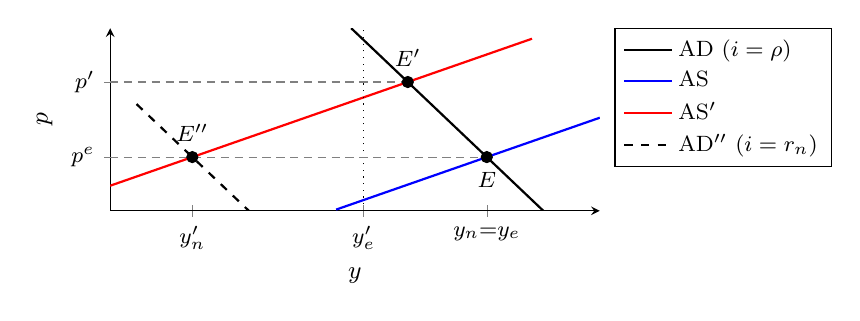
\begin{tikzpicture}
\pgfmathsetmacro{\Fsg}{0.5}\pgfmathsetmacro{\Fkp}{(1-0.75)*(1/0.5+0.2)/0.75}% sigma, kappa (alpha=.75, eta=.2)
\pgfmathsetmacro{\Fyn}{((1+0.2)*(-3)-5)/(1/0.5+0.2)}\pgfmathsetmacro{\Fye}{(1+0.2)*(-3)/(1/0.5+0.2)}% a=-3, mu=5
\pgfmathsetmacro{\FyE}{\Fsg*\Fkp*\Fyn/(1+\Fsg*\Fkp)}\pgfmathsetmacro{\FpE}{-\Fkp*\Fyn/(1+\Fsg*\Fkp)}
\begin{axis}[width=7.8cm,height=3.9cm,xmin=-5,xmax=1.5,ymin=-1.5,ymax=3.6,axis lines=left,
  xlabel={$y$},ylabel={$p$},xtick={\Fyn,\Fye,0},xticklabels={$y_n'$,$y_e'$,$y_n{=}y_e$},
  ytick={0,\FpE},yticklabels={$p^e$,$p'$},tick label style={font=\footnotesize},
  label style={font=\small},legend style={font=\footnotesize},legend cell align=left,legend pos=outer north east]
\addplot[thick,black,domain=-1.8:0.75]{-x/\Fsg};
\addplot[thick,blue,domain=-2:1.5]{\Fkp*x};
\addplot[thick,red,domain=-5:0.6]{\Fkp*(x-\Fyn)};
\addplot[thick,black,dashed,domain=-4.65:-3.15]{-(x-\Fyn)/\Fsg};
\legend{AD ($i=\rho$),AS,AS$'$,AD$''$ ($i=r_n$)}
\addplot[only marks,mark=*] coordinates {(0,0) (\FyE,\FpE) (\Fyn,0)};
\draw[dotted] (axis cs:\Fye,-1.5) -- (axis cs:\Fye,3.6);
\draw[gray,densely dashed] (axis cs:-5,\FpE) -- (axis cs:\FyE,\FpE) (axis cs:-5,0) -- (axis cs:0,0);
\node[font=\footnotesize,anchor=south,yshift=2pt] at (axis cs:\FyE,\FpE) {$E'$};
\node[font=\footnotesize,anchor=south,yshift=2pt] at (axis cs:\Fyn,0) {$E''$};
\node[font=\footnotesize,anchor=north,yshift=-2pt] at (axis cs:0,0) {$E$};
\end{axis}
\end{tikzpicture}
\end{center}
\intuicao{The productivity half moves $y_n$ and $y_e$ alike; the markup half moves only $y_n$. Both raise $r_n$, so $i=\rho$ sits below the price-stabilizing rate.}
\refbib{Benigno (2015), \S\S5--7, pp.~509--514; natural rate on p.~513.}
\rubrica{
\item Gap formula derived: 1 pt. Shock reduced to one of its halves: max.\ half of the item.
\item Both policies and the condition on the sign of $y-y_e'$: 1 pt; a sign without the condition: 0 for this line.
\item Graph (scored on its own): axes, AS$'$ through $(y_n',p^e)$, AD and AD$''$, $E'$, $E''$ and $y_e'$: 1 pt.
}
\end{sol}

\textbf{e)} (3 points) \emph{Parameter analysis.} For the markup shock alone ($\mu>0$, $a=0$, $i=\rho$), find $y$, $p-p^e$ and the natural
gap $y-y_n$ in closed form, sign their responses to $\alpha$, $\sigma$, $\eta$ and $\mu$ with proofs in a table, give the limits $\alpha\to0$
and $\alpha\to1$, and read the results.
\resolespaco
\begin{sol}
\passo{closed forms}{With $a=0$: $y_e=0$, $y_n=-\frac{\sigma\mu}{1+\sigma\eta}$. With $\xi\equiv\frac{1-\alpha}{\alpha}$ (free of $\sigma,\eta$), $\sigma\kappa=\xi(1+\sigma\eta)$ and
$\Delta\equiv1+\xi(1+\sigma\eta)$, (d) at $i=\rho$ gives $y=\frac{\sigma\kappa y_n}{1+\sigma\kappa}=-\frac{\sigma\mu\xi}{\Delta}$, $p-p^e=-\frac{\kappa y_n}{1+\sigma\kappa}=\frac{\mu\xi}{\Delta}$, $y-y_n=\frac{\sigma\mu}{(1+\sigma\eta)\Delta}$.}
\passo{signs}{Differentiating ($\partial_\xi y_n=0$, $\partial_\sigma y_n=-\frac{\mu}{(1+\sigma\eta)^2}$, $\partial_\eta y_n=\frac{\sigma^2\mu}{(1+\sigma\eta)^2}$):
\[\begin{aligned}
\partial_\xi y&=-\tfrac{\sigma\mu}{\Delta^2}, & \partial_\xi(p-p^e)&=\tfrac{\mu}{\Delta^2}, & \partial_\xi(y-y_n)&=-\tfrac{\sigma\mu}{\Delta^2},\\
\partial_\sigma y&=-\tfrac{\mu\xi(1+\xi)}{\Delta^2}, & \partial_\sigma(p-p^e)&=-\tfrac{\mu\eta\xi^2}{\Delta^2}, & \partial_\sigma(y-y_n)&=\tfrac{\mu(1+\xi-\xi\sigma^2\eta^2)}{(1+\sigma\eta)^2\Delta^2},\\
\partial_\eta y&=\tfrac{\sigma^2\mu\xi^2}{\Delta^2}, & \partial_\eta(p-p^e)&=-\tfrac{\sigma\mu\xi^2}{\Delta^2}, & \partial_\eta(y-y_n)&=-\tfrac{\sigma^2\mu[1+2\xi(1+\sigma\eta)]}{(1+\sigma\eta)^2\Delta^2}.
\end{aligned}\]
As $d\xi/d\alpha=-1/\alpha^2<0$, the $\alpha$-signs are opposite to the $\xi$-signs (in $\kappa$: $\partial_\kappa\frac{\kappa}{1+\sigma\kappa}=\frac{1}{(1+\sigma\kappa)^2}>0$); all
results are proportional to $\mu$; and $\partial_\sigma(y-y_n)>0$ iff $1+\xi>\xi\sigma^2\eta^2$, i.e.\ $\sigma^2\eta^2<\frac{1}{1-\alpha}$.}
\begin{center}
\begin{tabular}{lcccc}
\toprule
 & $\alpha$ & $\sigma$ & $\eta$ & $\mu$ \\
\midrule
$y_n$ & $0$ & $-$ & $+$ & $-$ \\
$y$ \ $(=y-y_e)$ & $+$ & $-$ & $+$ & $-$ \\
$p-p^e$ & $-$ & $-$ & $-$ & $+$ \\
$y-y_n$ & $+$ & $+$ iff $\sigma\eta<(1-\alpha)^{-1/2}$ & $-$ & $+$ \\
\bottomrule
\end{tabular}
\end{center}
\passo{limits}{$\alpha\to1$ ($\kappa\to0$): $y\to0$, $p\to p^e$, $y-y_n\to-y_n$ (output is demand-determined and the AD has not moved). $\alpha\to0$
($\kappa\to\infty$): $y\to y_n$, $p-p^e\to\frac{\mu}{1+\sigma\eta}$, $y-y_n\to0$. Knife edge: $1+\xi-\xi\sigma^2\eta^2$ falls in $\sigma$ and vanishes once, at
$\sigma^*=\frac{1}{\eta\sqrt{1-\alpha}}$, where the natural gap peaks.}
\passo{reading}{With $i$ held, demand pins output down: rigid prices shield output from a cost shock, flexible ones pass it into prices
($y\to y_n$). As $y_e$ is fixed, more flexibility enlarges the efficiency loss and the price surprise while shrinking the natural gap, which
is thus no welfare criterion. A higher $\sigma$ turns the price surprise into a larger fall in demand and deepens the fall of $y_n$ (so the
natural gap first widens, then narrows); a higher $\eta$ shrinks the fall of $y_n$ and steepens the AS, so output and prices move less.}
\intuicao{Output absorbs the share $\frac{\sigma\kappa}{1+\sigma\kappa}$ of the fall in $y_n$, rising in $\kappa$ and $\sigma$.}
\refbib{Benigno (2015), \S7, pp.~513--514; Romer (2012), problem 6.16.}
\rubrica{
\item Closed forms: 1 pt.
\item Signs proved, limits and the $\sigma$ condition: 1 pt; a sign or limit without proof: 0 for that entry.
\item Table and reading: 1 pt; signs without proofs or without reading: max.\ half of the item.
}
\end{sol}
